\documentclass{sig-alternate}
\usepackage{color}
\usepackage[colorinlistoftodos]{todonotes}

\linespread{.99}

%%%%% Uncomment the following line and comment out the previous one
%%%%% to remove all comments
%%%%% NOTE: comments still occupy a line even if invisible;
%%%%% Don't write them as a separate paragraph
%\newcommand{\mycomment}[1]{}
\newcommand{\ceil}[1]{\lceil #1 \rceil}

\begin{document}

% --- Author Metadata here ---
%%% REMEMBER TO CHANGE THE SEMESTER AND YEAR AS NEEDED
\conferenceinfo{UMM CSci Senior Seminar Conference, April 2016}{Morris, MN}

\title{Parallel BVH Construction for Real-Time Ray Tracing}

\numberofauthors{1}

\author{
% The command \alignauthor (no curly braces needed) should
% precede each author name, affiliation/snail-mail address and
% e-mail address. Additionally, tag each line of
% affiliation/address with \affaddr, and tag the
% e-mail address with \email.
\alignauthor
Aaron Lemmon\\
	\affaddr{Division of Science and Mathematics}\\
	\affaddr{University of Minnesota, Morris}\\
	\affaddr{Morris, Minnesota, USA 56267}\\
	\email{lemmo031@morris.umn.edu}
}

\maketitle
\begin{abstract}

% The current paper format *only* allows inline comments using the todo
% macro. That's kind of a bummer, and it would be neat if someone figured
% out how to change the acmconf style to allow this. I suspect it isn't *hard*
% but there are quite a few details that have to be sorted out in synchrony.
The rise in popularity of interactive graphical applications, such as video games, has motivated innovations in rendering 3D scenes in real time. The ray tracing technique is well-suited for generating realistic images of scenes that feature shadows, reflections, and refractions. Historically, ray tracing has been too slow for real-time applications since it is computationally intensive. However, ray tracing performance can be greatly improved by using the bounding volume hierarchy (BVH) acceleration data structure to store scene information for each frame. Researchers have strived to minimize the combined time of both constructing and using BVHs for ray tracing. This paper provides an overview of ray tracing with BVHs and presents a recently developed method for constructing them in parallel on a GPU.
	
\end{abstract}

\keywords{computer graphics, ray tracing, parallel computing, bounding volume hierarchies, Morton codes}

\section{Background}
\label{sec:background}

In 3D computer graphics, objects are made up of a collection of \emph{primitives}, which are usually simple geometric shapes like triangles. A 3D \emph{scene} consists of all the primitives that construct it. Figure~\ref{fig:dolphin} depicts a scene with a dolphin that clearly shows the component triangles. In order to depict a scene on a display, the pixels of the display must be colored to create an image. A technique called \emph{ray tracing} can be used to color the pixels in a way that can accurately portray shadows, reflections, and refractions in a scene~\cite{Viitanen:2015}. Ray tracing achieves this by determining how light travels in a scene from the light sources, reflecting or refracting off objects, and meeting the viewer~\cite{Whitted:1980}. Figure~\ref{fig:glasses} shows the high degree of photorealism that ray tracing can achieve.

\begin{figure}
\centering
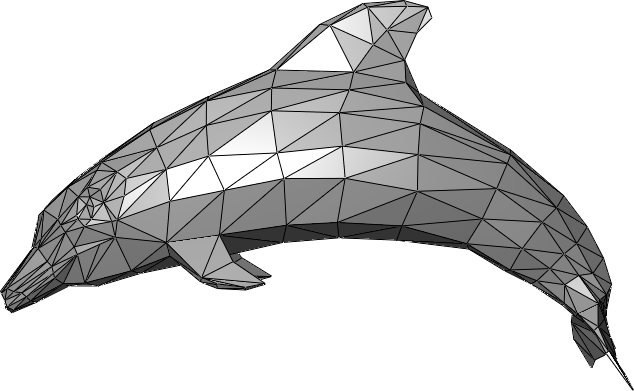
\psfig{file=Dolphin_triangle_mesh.png,width =3in}
\caption{A simple scene containing a dolphin constructed from triangle primitives~\cite{wiki:mesh}.}
\label{fig:dolphin}
\end{figure}

Since many rays from a light source may not ultimately reach the viewer, it is more practical to start from the viewer and trace paths of light backward. Figure~\ref{fig:ray_diagram} shows that for every pixel on a display, a ray is traced from the viewpoint through the pixel and into the 3D scene. When a ray intersects with the first primitive in its path it recursively generates more rays in directions that will contribute to an appearance of reflections, refrations, or shadows~\cite{Whitted:1980}. While ray tracing can create highly realistic images, the process of tracing a large number of rays for a 3D scene with many primitives on a high resolution display can take a long time.

\begin{figure}[t]
\centering

\psfig{file=Glasses_800_edit.png,width =3in}
\caption{A ray traced scene featuring shadows on the wall and beneath the glasses, reflections on the glossy surfaces of the glasses, and refractions through the glass stems and ice cube~\cite{wiki:rayTracing}.}
\label{fig:glasses}
\end{figure}

Ray tracing a single frame of a 3D scene can involve testing for intersections of billions of rays against millions of primitives~\cite{Gribble:2012, Wald:2007}. To speed up this process, acceleration data structures can be used to organize the primitives by their location so that only the primitives near a given ray need to be checked for intersection with that ray. Acceleration data structures usually take the form of a tree: the top node represents the entire 3D volume of the scene and the children of every node divide up the volume of their parent node into subsections. Although these acceleration data structures speed up ray intersection testing, the time it takes to build these trees can negatively impact performance~\cite{Garanzha:2011}. This is especially apparent in scenes with moving objects since the acceleration data structures need to be rebuilt or updated to accurately reflect the new locations of objects~\cite{Wald:2007}.

The research discussed here addresses methods for building and maintaining acceleration data structures in a way that minimizes the combined time spent constructing the data structure and using it to test for ray intersections. In particular, parallel computing on the \emph{graphics processing unit} (GPU) can decrease the time spent building an acceleration data structure. Efficient acceleration data structures allow for ray tracing scenes with motion in real time.

\begin{figure}
\centering
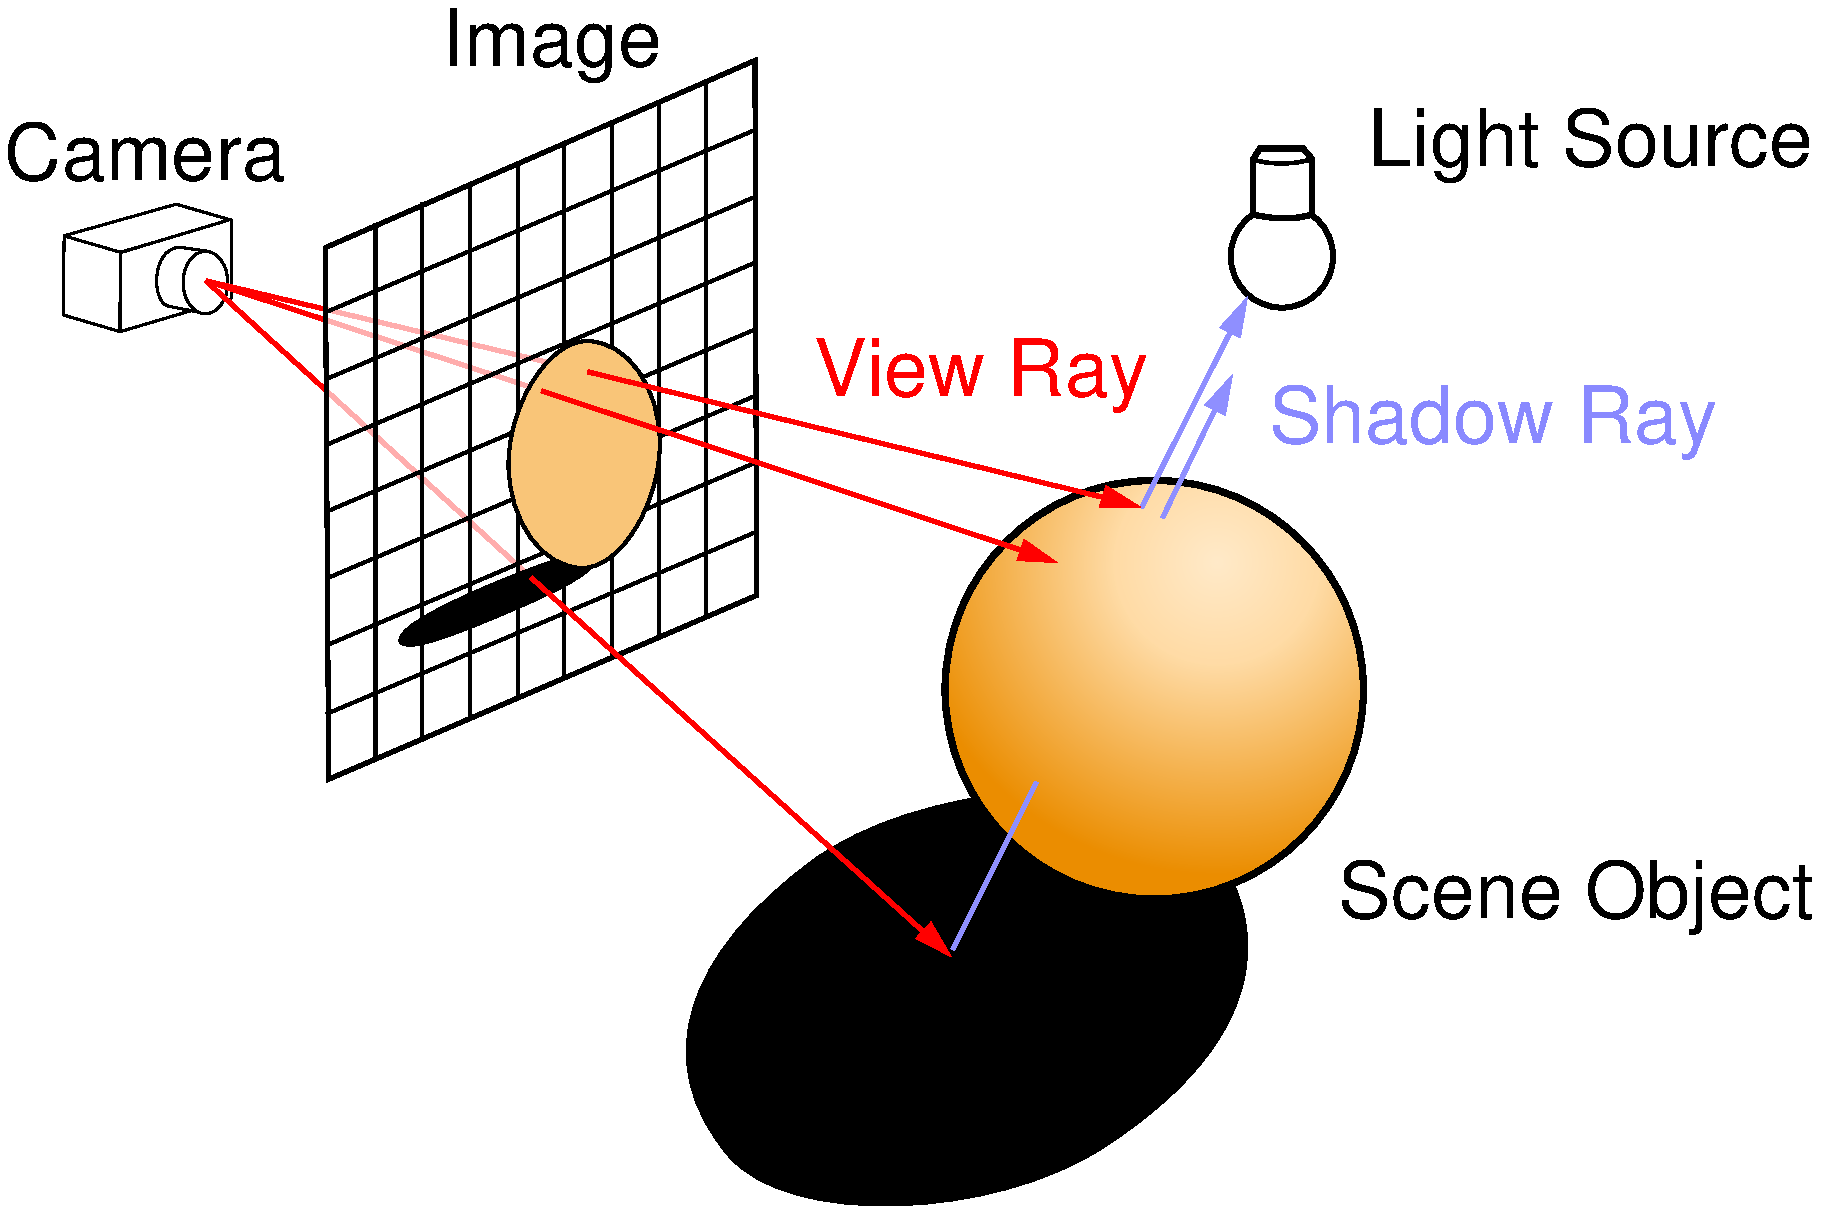
\psfig{file=Ray_trace_diagram.pdf,width =3in}
\caption{For each pixel of the image plane, a ray is cast through and tested for intersection with objects in the scene. When intersections occur, the angle of reflection is calculated and a new ray is sent out. Eventually, if a ray intersects with a light source, the color information propagates back to the pixel~\cite{Gribble:2012, wiki:rayTracing}.}
\label{fig:ray_diagram}
\end{figure}

\section{Acceleration Data Structures}
\label{sec:accel}

If primitives of a scene are stored in a data structure that identifies their location in the scene, then a ray only needs to check for intersections with objects located in the parts of the scene the ray is passing through. This can drastically improve the performance of intersection testing for each ray~\cite{wiki:rayTracing}.

A way to make intersection tests easier to calculate is to surround primitives with \emph{bounding boxes}. A bounding box is a box that completely contains its contents as tightly as possible. A common approach is to use \emph{axis-aligned bounding boxes} (AABBs), which are aligned with the axes of the scene as a whole. It is much simpler to test for ray intersections with AABBs than with the items they contain. If a ray does not intersect with an object's AABB, then it cannot intersect with the object itself. However, if it does intersect with the AABB, then a more costly check must be made to test for intersection with the contained object. Overall, using AABBs can reduce the cost of testing for intersections since a ray misses many more objects than it hits.

%\begin{figure}[h]
%\centering
%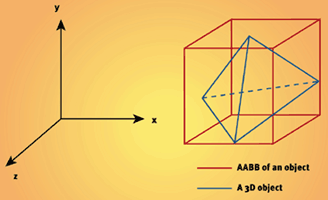
\psfig{file=aabb.png,width =3in}
%\caption{An axis aligned bounding box containing an object constructed from four triangles. Note that the box is fitted as tightly as possible and the edges of the box lie parallel to the axes of the scene.}
%\label{fig:AABB}
%\end{figure}

% From http://gimpact.sourceforge.net/manual/manual_figures/aabb.gif

\emph{Bounding volume hierarchies} (BVHs) extend the idea of AABBs to a binary tree data structure as shown in Figure~\ref{fig:BVH}. The root node of a BVH is an AABB that surrounds all the primitives in the scene. Every parent node has two child nodes, each of which is an AABB that surrounds its share of the primitives surrounded by the parent node. By continually separating volumes into smaller volumes, it becomes possible to group close primitives together~\cite{Wald:2007}. The lower nodes on the tree give more precise location information than the higher nodes. The leaves of the tree are AABBs that surround a single primitive~\cite{wiki:bvh}. As opposed to other types of acceleration data structures, BVHs define the volumes by the objects they contain rather than splitting volumes and then determining which objects should go in each node~\cite{Wald:2007}.

\begin{figure}[t]
\centering
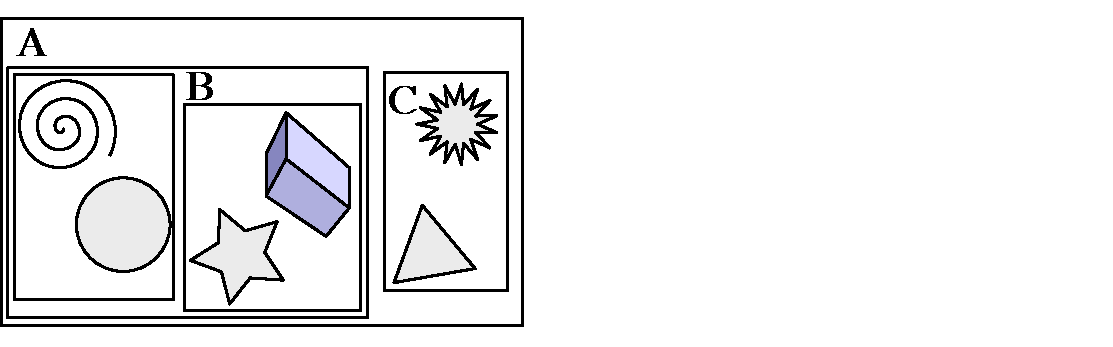
\psfig{file=bvh_diagram.pdf,width =3in}
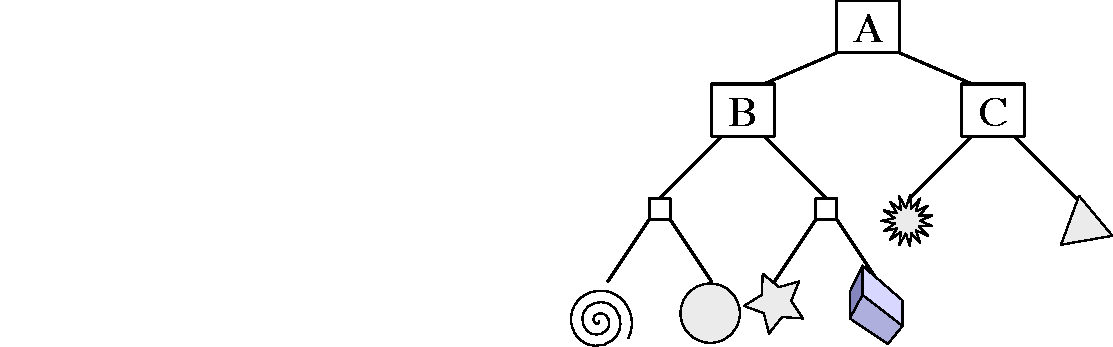
\psfig{file=bvh_tree.pdf,width =3in}
\caption{Top: A 2D scene with rectangles as bounding boxes. Bottom: One possible BVH configuration for the 2D scene. Note that each internal node has exactly two children and that objects that are close in the scene are also close in the BVH tree~\cite{wiki:bvh}.}
\label{fig:BVH}
\end{figure}

Searching for a ray intersection with objects in a BVH occurs in a top-down manner. First, the ray is tested against the root of the tree to check if it intersects with the scene. If it does, then both of the root's children are checked for intersection. If the ray misses a child node, then the entire subtree rooted at that node can be eliminated from the rest of the search, since the objects contained within the node will also not intersect. However, in the case that the ray intersects both children, the search must continue down both subtrees~\cite{Gribble:2012}. In the best-case scenario, where that does not happen, the number of checks will be approximately the log of the number of total primitives. Ray tracing with a BVH structure can therefore greatly reduce the number of intersection checks performed per ray~\cite{wiki:bvh}. 

\section{BVH Construction}
\label{sec:bvh}

In order to speed up the construction of BVHs for real-time ray tracing, Tero Karras~\cite{Karras:2012} has developed a method based upon earlier work by Garanzha et al.~\cite{Garanzha:2011} for constructing an entire BVH tree in parallel on a GPU. The method follows a series of four main steps. The method first assigns a value called a \emph{Morton code} to each primitive based upon its location in the scene. The Morton codes are then sorted. Next, a \emph{binary radix tree} (defined in Section~\ref{sec:brtFundamentals}) is constructed in parallel, which arranges close primitives near each other in the tree. The last step fits an AABB around the contents of each node in the binary radix tree in parallel to form the final BVH~\cite{Karras:2012}. The next sections will cover each of these steps in more detail.

\subsection{Morton Codes}
\label{sec:mortonCodes}

The location of each primitive in the scene can be represented by the $x$, $y$, and $z$ coordinates of the center of its AABB~\cite{Viitanen:2015, Wald:2007}. The Morton code of a primitive combines the coordinates into a single value by interleaving the binary representations of the $x$, $y$, and $z$ coordinates~\cite{Garanzha:2011}. A Morton code has the form \begin{math}X_{0}Y_{0}Z_{0}X_{1}Y_{1}Z_{1}\dots\end{math} where the $x$ coordinate is represented as the binary digits \begin{math}X_{0}X_{1}X_{2}\dots\end{math}, and similarly for the $y$ and $z$ coordinates~\cite{Karras:2012}.

Figure~\ref{fig:MortonCodeFigure} shows a two dimensional scene area with the Morton codes of each coordinate location. The lowest valued Morton code appears in the upper-left corner of the scene where both coordinates are zero. The zigzag pattern on the image shows the sequence of increasing Morton codes, which ultimately ends with the highest value in the lower-right corner. Every primitive in the scene is assigned a Morton code based on its location, and each code (paired with a reference to its primitive) is added to an array. Primitives that share a common location will be assigned the same Morton code specifying that location, while Morton codes for empty areas of the scene will be unused~\cite{Karras:2012, Viitanen:2015}.

Note that in Figure~\ref{fig:MortonCodeFigure} all codes that start with a 0 bit are located in the upper half of the scene, and within that section all codes that have a 0 as the second bit are located on the left half of that section~\cite{Garanzha:2011}. This property of Morton codes allows primitives that are near each other to have long \emph{common prefixes} between their Morton codes, which is important for the binary radix tree construction. The array of Morton codes is sorted in order to group the codes by common prefixes~\cite{Viitanen:2015}. Note that the actual primitives in the scene are not moved.

\begin{figure}
\centering
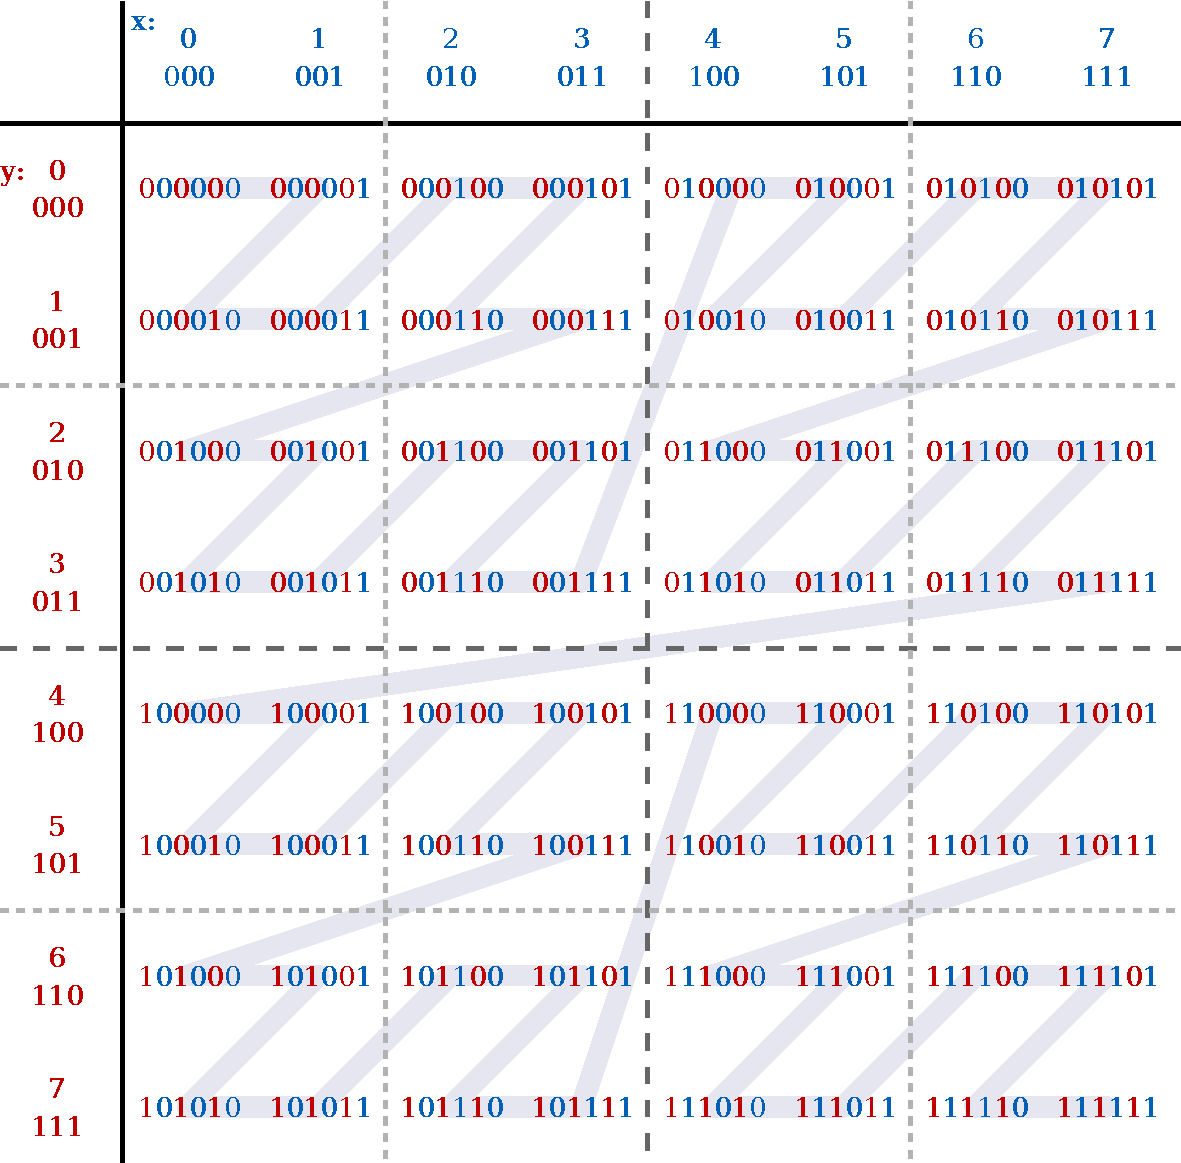
\psfig{file=Z-curve.pdf,width =3in}
\caption{Morton codes for each location in a 2D scene. Notice that each Morton code is made by interleaving the bits of the $x$ (blue) and $y$ (red) coordinates for its location~\cite{wiki:morton}.}
\label{fig:MortonCodeFigure}
\end{figure} 

\subsection{Binary Radix Tree Construction}
\label{sec:brts}

\subsubsection{Binary Radix Tree Fundamentals}
\label{sec:brtFundamentals}

The array of sorted Morton codes can be thought of as a set of $n$ bit string keys \begin{math}k_{0},\dots,k_{n-1}\end{math} where $n$ represents the number of primitives in the scene. A binary radix tree organizes the keys under a tree structure where the leaves are the keys and the internal nodes represent common binary prefixes of the keys. Figure~\ref{fig:BinaryRadixTree} shows an example of the binary radix tree for a set of eight binary keys, which are the Morton codes of primitives in a scene. Each key is a leaf node, and each internal node represents the longest common prefix shared by all the keys under it. These prefixes are always shorter than the full Morton codes, and longer prefixes represent a narrower set of locations in the scene. Every internal node always has exactly two children: the left child has the common prefix of the its parent followed by a 0 bit, and the right child has the same common prefix but followed by a 1 bit~\cite{Karras:2012}. As an example, the left child of the root in Figure~\ref{fig:BinaryRadixTree} has the prefix ``00'', thus every key under its left child begins with ``000'' and every key under its right child begins with ``001''. Since every internal node has exactly two children, a binary radix tree with $n$ leaf nodes will always have exactly $n-1$ internal nodes~\cite{Wald:2007}.

Every key in a binary radix tree must be unique, but duplicate Morton codes could exist if the primitives are extremely close. To ensure uniqueness, the binary representation of each key's index in the array can be concatenated onto the end of the key. These concatenations do not need to be stored, but can be performed as needed when comparing identical keys~\cite{Karras:2012}. For example, if two keys both have the Morton code ``010'' and they are stored at indices (in binary) 000 and 001, then the index concatenation will result in the unique values ``010000'' and ``010001''. 

\begin{figure}
\centering
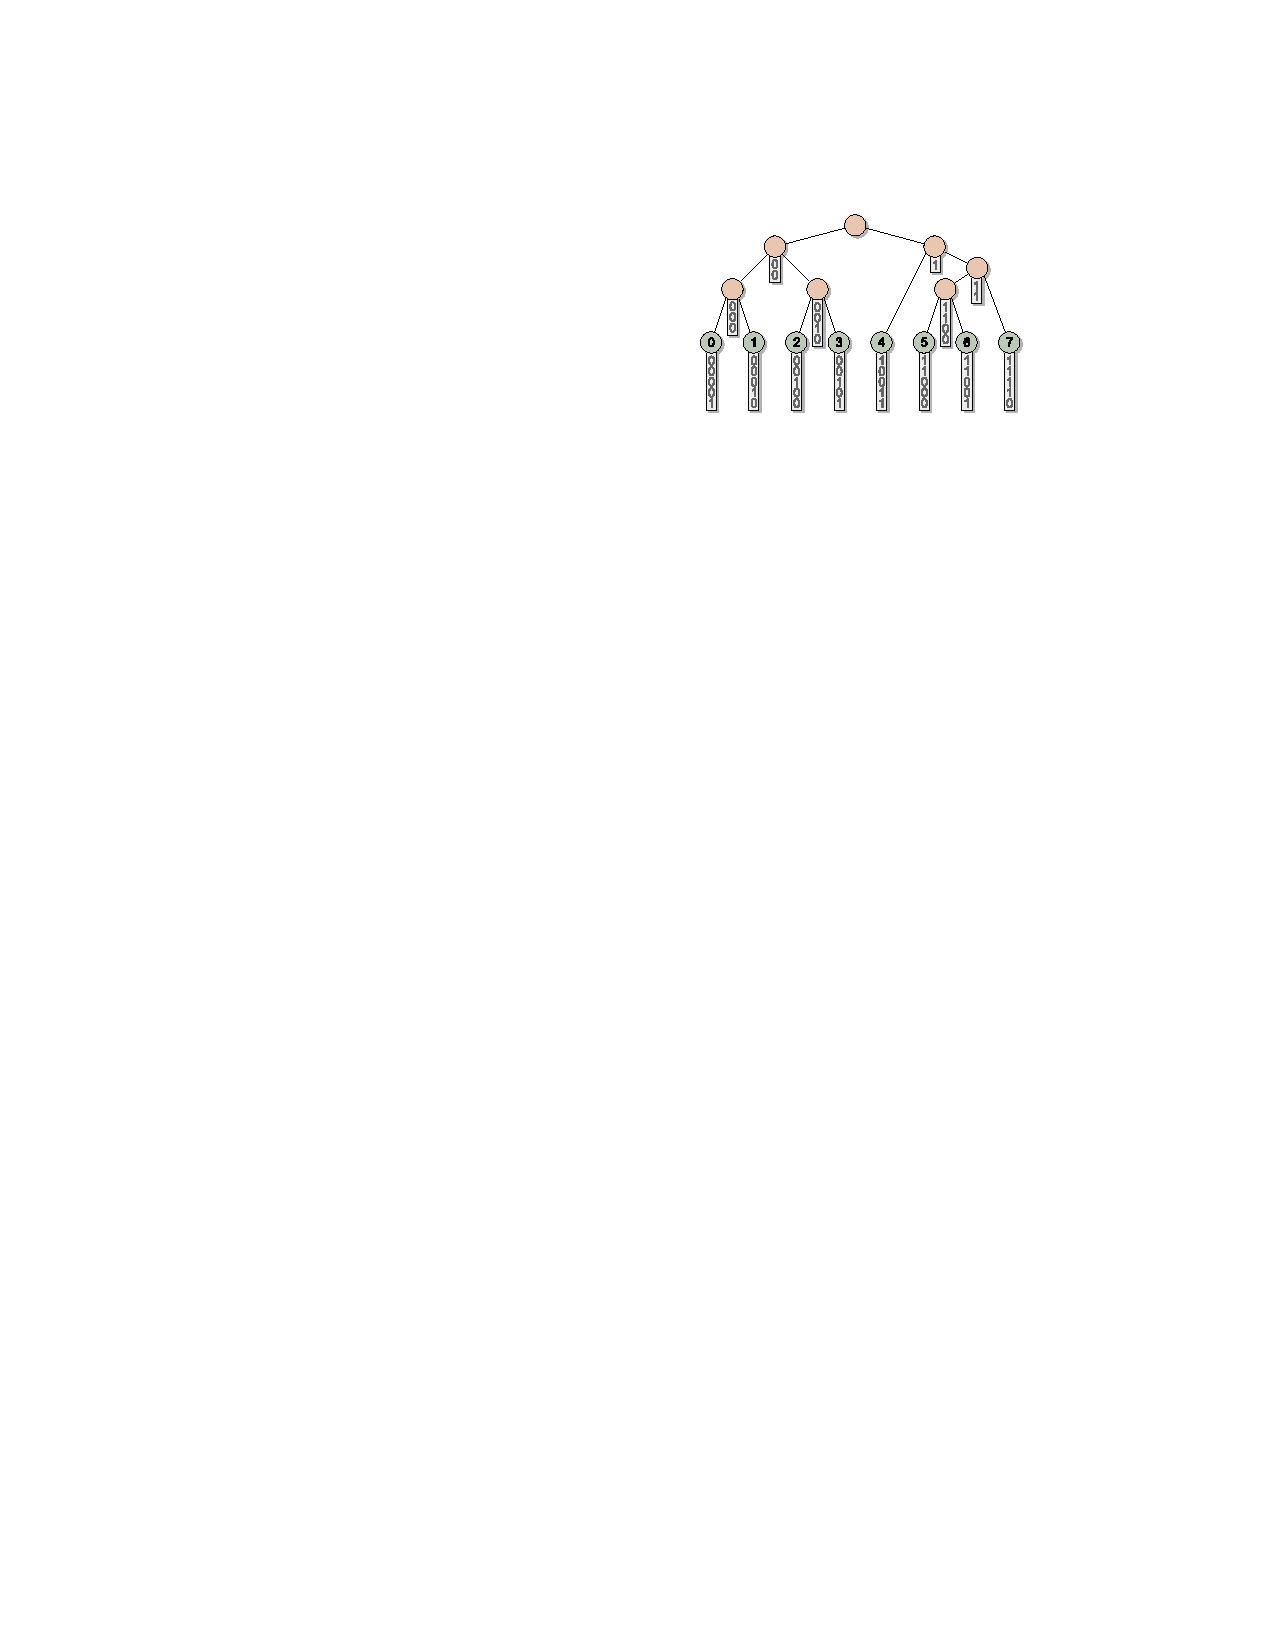
\psfig{file=BinaryRadixTree.pdf,width =3in}
\caption{An ordered binary radix tree. There are eight leaf nodes containing 5-bit keys which appear in lexicographical order. Each internal node covers a linear range of keys with a common prefix displayed directly beneath the node. The range of keys covered by an internal node is partitioned into two subranges according to their first differing bit; these two subranges are represented by the two children of the internal node~\cite{Karras:2012}.}
\label{fig:BinaryRadixTree}
\end{figure}

\subsubsection{Binary Radix Tree Properties}
\label{sec:brtProperties}

In order to create every internal node of the binary radix tree construction in parallel, it must be possible to determine three properties about a node. These properties include the range of keys that a node covers, the length of the longest common prefix of those keys, and what the node's children are. Additionally, these must be determined without depending on the work done in any other internal nodes since all the nodes will be working in parallel. This section will cover the three important properties of an internal node and Sections~\ref{sec:setup} and \ref{sec:algorithm} will discuss the binary radix tree construction.

The keys covered by an internal node can be represented as a linear range $[i,j]$. Using Figure~\ref{fig:BinaryRadixTree} as an example, the root node covers keys 0 through 7, so it can be represented as the range $[0,7]$. Its left child can be represented as $[0,3]$ and its right child as $[4,7]$.

~

The length of the longest common prefix between two keys, $k_{i}$ and $k_{j}$, is denoted by $\delta(i,j)$. For example, the longest common prefix between key 0 and key 3 in Figure~\ref{fig:BinaryRadixTree} is ``00'', which has a length of two digits. So $\delta(0,3)$ is 2.

The prefix for each internal node can be determined by solely inspecting the first key and last key in the node's key range. This is because all keys between the first key and last key will also share the same prefix since all keys are in lexicographical order~\cite{Karras:2012}. As an example, the left child of the root in Figure~\ref{fig:BinaryRadixTree} covers keys 0 through 3. By only looking at keys 0 and 3, it can be determined that they share the prefix ``00''. All keys between 0 and 3 will also start with ``00'', otherwise they would not fall in that range.

An internal node partitions its range of keys into two subranges for its children according to the first differing bit among the keys. For example, the left child of the root in Figure~\ref{fig:BinaryRadixTree} covers keys 0 through 3 with a common prefix of ``00''. This node will divide its keys among its children based on the value of the third bit of the keys, since the third bit comes directly after the common prefix. All keys in the range with 0 as the third bit will belong under the left child and the keys with 1 as the third bit will belong under the right child. The index of the last key where the differing bit is 0 is called the \emph{split position} for the node, and is denoted by $\gamma$. If the range of keys covered by a node is $[i,j]$, then the split position can be anything from $i$ to $j-1$. The split position cannot occur at $j$, since the differing bit must be a 1 for key $j$. The split position for the left child of the root in Figure~\ref{fig:BinaryRadixTree} is 1 because key 1 is the last key in the range $[0,3]$ that starts with ``000''. The next key must start with ``001''. The subrange $[i,\gamma]$ represents the range of keys covered by the left child and the subrange $[\gamma+1,j]$ represents the range covered by the right child~\cite{Karras:2012}.

For an internal node with range $[i,j]$, the equality $\delta(\gamma,\gamma+1)=\delta(i,j)$ always holds true and is important for finding the the split position. In fact, $k_{\gamma}$ and $k_{\gamma+1}$ is the only pair of adjacent keys in the range where the prefix length of the two keys is equal to the prefix length of the entire range. Pairs of adjacent keys to the left of the split position will have a longer common prefix than the range since they all have 0 in the differing bit position. Adjacent keys to the right of the split position are analogous, but with all having a 1 in the differing bit position.

\subsubsection{Setup for Binary Radix Tree Construction}
\label{sec:setup}

It is possible to construct a binary radix tree by starting with the root node, finding the first differing bit in the keys, creating the child nodes, then handling each child recursively. However, this is not parallel because a node cannot be created until all of its ancestors have been created. Parallel construction can be achieved by creating a connection between internal node indices and keys through a particular tree setup. This is done by assigning indices to internal nodes in a way that enables finding their children without depending on that node's ancestors being finished~\cite{Karras:2012}.

\begin{figure}
\centering
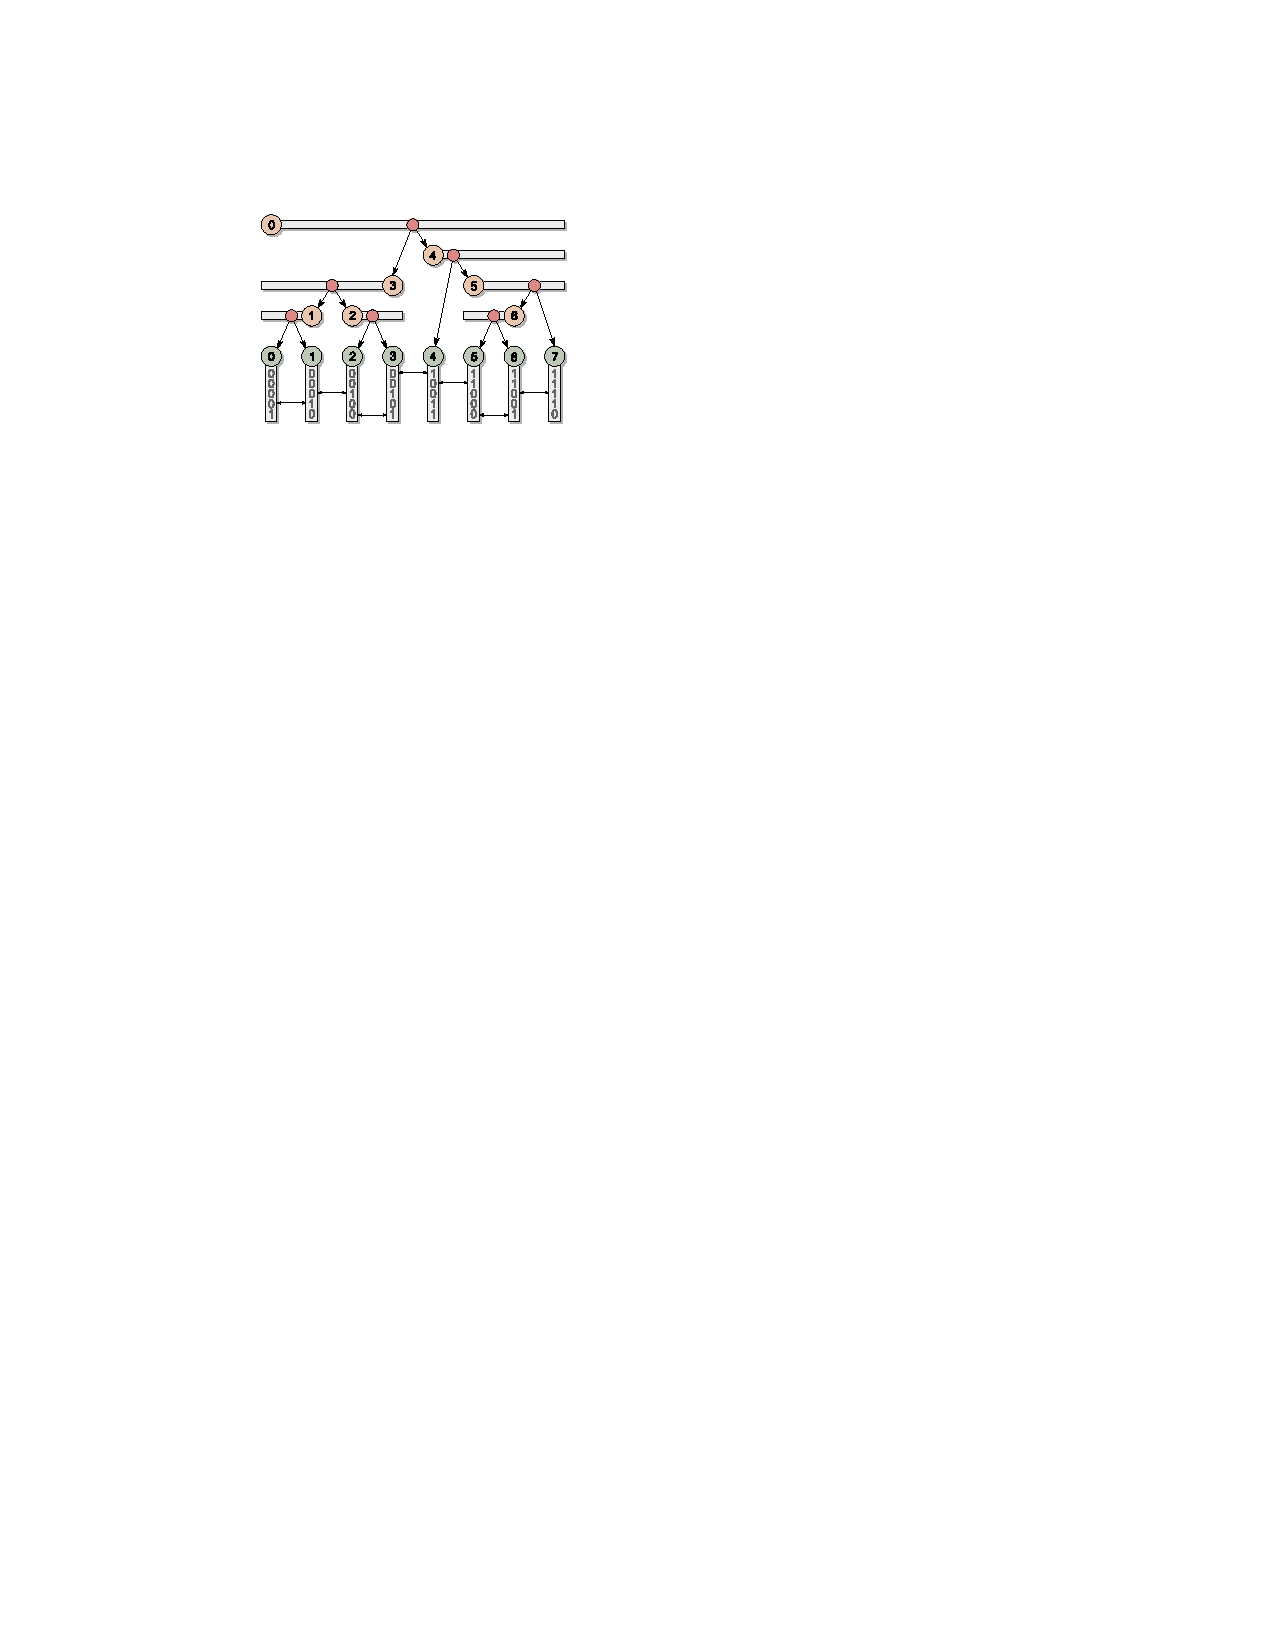
\psfig{file=radix_tree_arrays.pdf,width =3in}
\caption{This figure shows the storage locations of nodes for the binary radix tree displayed in Figure~\ref{fig:BinaryRadixTree}. The internal nodes have been assigned indices from 0 to 6 and are lined up with leaf nodes with the same indices. The range of keys covered by each internal node is shown as a horizontal bar, and a tiny red circle lies immediately after each node's split position~\cite{Karras:2012}.}
\label{fig:BinaryRadixArrays}
\end{figure}

Figure~\ref{fig:BinaryRadixArrays} shows how the nodes of the binary radix tree from Figure~\ref{fig:BinaryRadixTree} will be stored. The leaf nodes and internal nodes are stored in two separate arrays, $L$ and $I$, respectively. The root will always be located at position $I_{0}$. The children of internal nodes are placed at an index according to their parent's split position. The left child is located at $L_{\gamma}$ if it is a leaf, or at $I_{\gamma}$ if it covers more than one key. Similarly, the right child is located at $L_{\gamma+1}$ or $I_{\gamma+1}$~\cite{Karras:2012}. For example, the split position of the root in Figure~\ref{fig:BinaryRadixArrays} is at index 3, so its left child is stored in $I_{3}$ and its right child is stored in $I_{4}$.

It is important to note that the index of every internal node is equal to the index of either its first or last key. The index of an internal node will be equal to the index of its first key if the node is a right child of its parent. Figure~\ref{fig:BinaryRadixArrays} shows that internal node 4 is a right child, that its index coincides with it first key (key 4), and that its range extends rightward. Conversely, internal node 3 is a left child, its index coincides with its last key (key 3), and its range extends leftward. More generally, if a node covers the range $[i,j]$, then its left child will be located at $\gamma$, which is the end of its range $[i,\gamma]$. The right child will be located at $\gamma+1$, which is the beginning of its range $[\gamma+1,j]$~\cite{Karras:2012}.

\subsubsection{Binary Radix Tree Construction Algorithm}
\label{sec:algorithm}

\begin{figure}
\centering
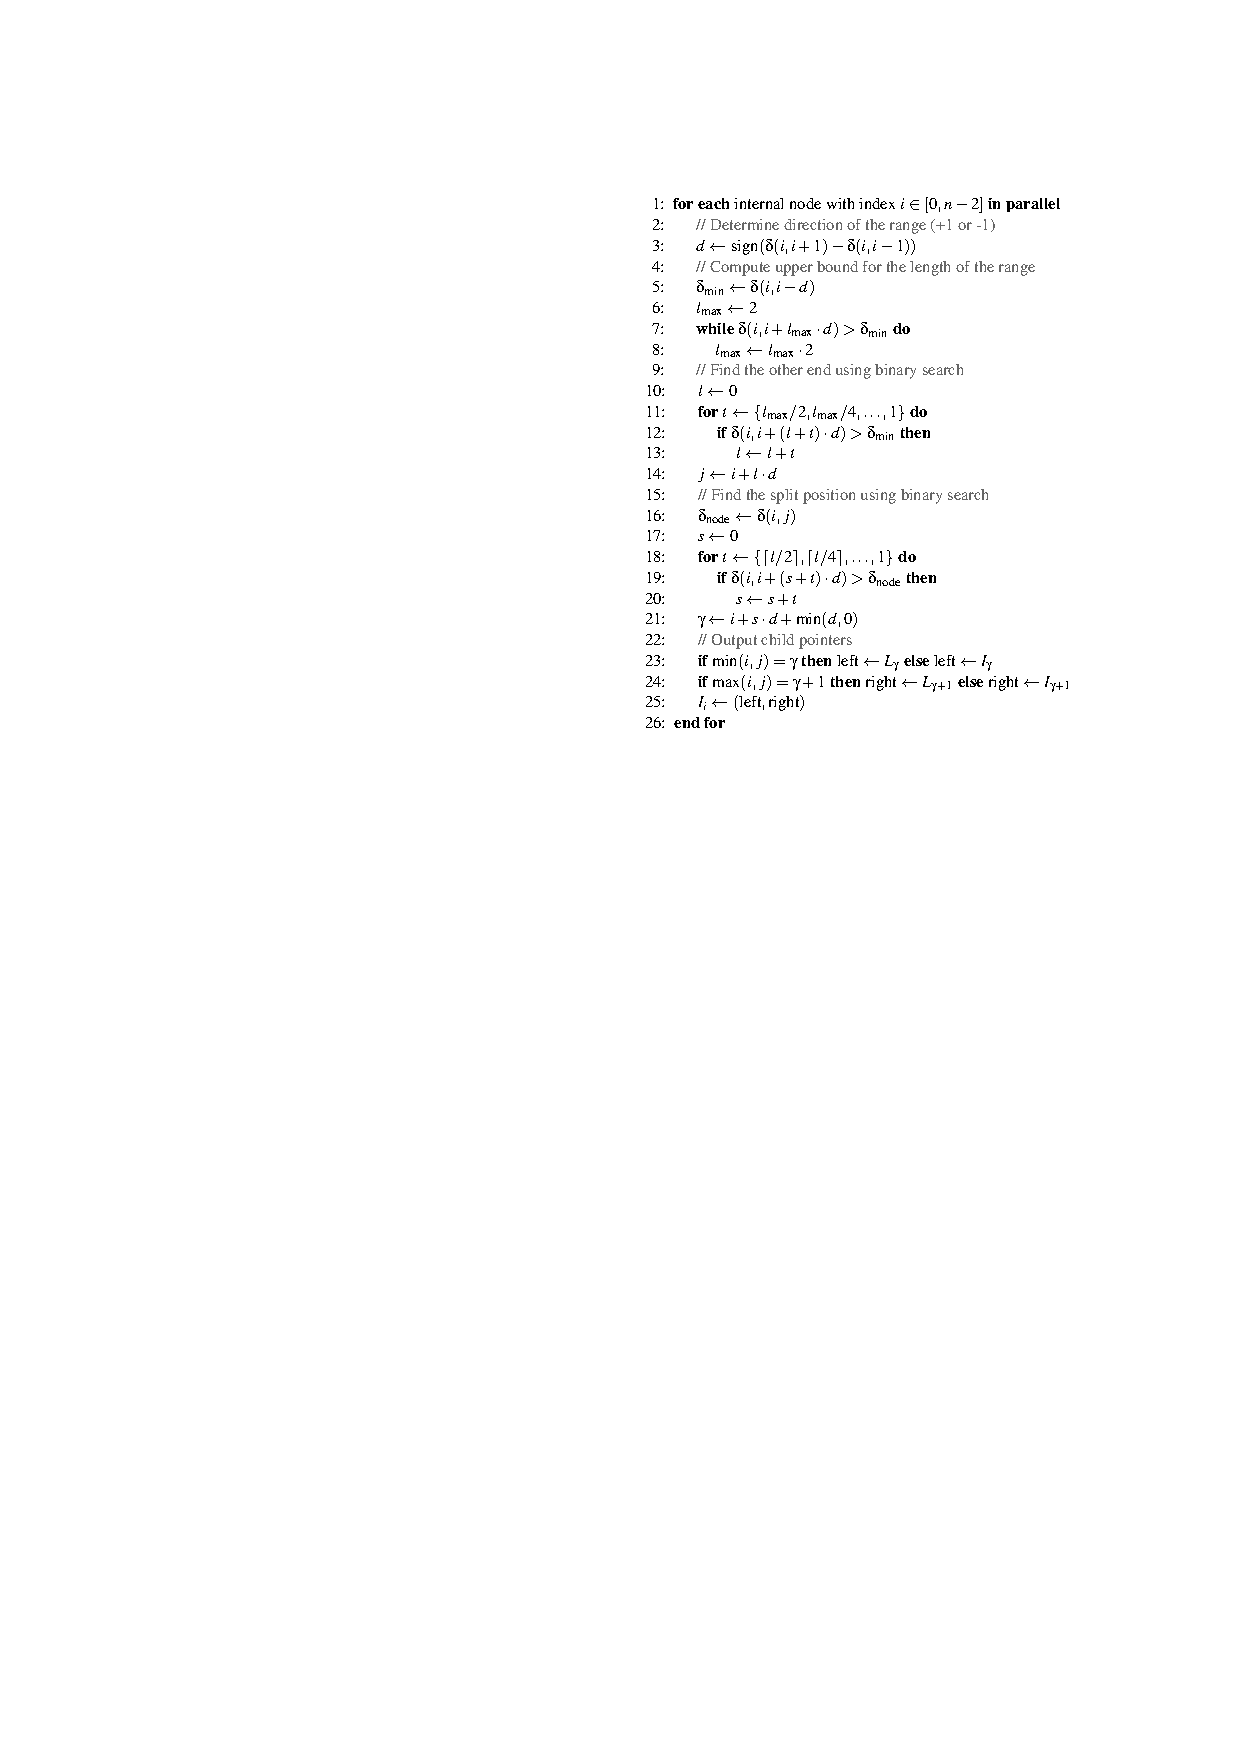
\psfig{file=PseudoCode.pdf,width =3in}
\caption{Pseudocode for binary radix tree construction. Note that if an out-of-bounds argument is passed to $\delta()$, it is defined to return -1~\cite{Karras:2012}.}
\label{fig:PseudoCode}
\end{figure}

The goal of the binary radix tree construction algorithm is to determine the range $[i,j]$ of keys covered by each internal node, as well as the indices of its children. One end of the range is given by the internal node's index, and the other end of the range can be found by examining the surrounding keys. The indices of the children can be found by locating the split position. The previous setup allows each internal node to be processed independently and in parallel with the other internal nodes~\cite{Karras:2012}. This section will explain the construction process using the pseudocode in Figure~\ref{fig:PseudoCode} as a reference.

Consider processing an internal node $I_{i}$, which is in the $i$th position of the array $I$. First, the direction the range extends (rightward or leftward) is calculated in line 3 of Figure~\ref{fig:PseudoCode}. If $d$ becomes $+1$ then the range extends rightward; if it becomes $-1$ then the range extends leftward~\cite{Karras:2012}. For example consider $I_2$, which covers keys 2 and 3 as shown in Figure~\ref{fig:BinaryRadixArrays}. In this example, $\delta(2,3) = 4$ while $\delta(2,1) = 2$, so the range of internal node 2 extends to the right since it shared a longer common prefix with its right neighbor.

The next task is to determine $j$ (handled in lines 5-14 in the pseudocode), which represents the index of the other end of the range $[i,j]$. For $I_2$, $j$ is 3 since the range of the internal node at index 2 covers keys 2 and 3. Every internal node covers at least two keys, therefore the two keys $k_i$ and $k_{i+d}$ must belong to $I_i$. The other neighboring key $k_{i-d}$ must belong to $I_{i-d}$. The two keys $k_i$ and $k_{i+d}$ share a common prefix that is different and longer than the prefix between $k_i$ and $k_{i-d}$. Let $\delta_{\textrm{min}}$ represent the value of $\delta(i, i-d)$. For $I_2$, $\delta_{\textrm{min}}$ equals 2, with the common prefix being ``00''. The value of $\delta_{\textrm{min}}$ is equivalent to the length of the prefix represented by the parent of the node currently under consideration. This fact is used to determine the index of $j$. For any $k_m$ belonging to $I_i$, the inequality $\delta(i,m)>\delta_{\textrm{min}}$ always holds true. Therefore, $\delta_{\textrm{min}}$ gives a lower bound for the length of the prefix for the section of keys covered by $I_i$. Thus, the index $j$ marking the other end of the range can be found by searching for the largest integer $l$ that satisfies $\delta(i, i+l \cdot d)>\delta_{\textrm{min}}$. Then $j$ will be the index $i+l \cdot d$~\cite{Karras:2012}.

Finding $j$ is achieved by first finding an exclusive power-of-two upper bound for $l$, denoted as $l_{\textrm{max}}$ (done in lines 6-8 of the pseudocode). As shown in Figure~\ref{fig:PseudoCode}, $l_{\textrm{max}}$ begins at 2 and is doubled until it becomes the upper bound for $l$. For example, for $I_5$, $l_{\textrm{max}}$ is doubled until it reaches 4. We can see from Figure~\ref{fig:BinaryRadixArrays} that $l$ is 2 for node 5 since it covers the keys $[5,5+2]$. Therefore, $l_{\textrm{max}}=4$ is the correct exclusive power-of-two upper bound for node 5~\cite{Karras:2012}.

Once the upper bound $l_{\textrm{max}}$ is determined, $l$ can be found by using binary search in the range $[0,l_{\textrm{max}}-1]$ (performed in lines 10-13). For example, for node 5, with $\delta_{\textrm{min}}=1$ and $l_{\textrm{max}}=4$, the loop goes through the range \{$2, 1$\}. $l$ starts at 0 and is incremented by 2 in the first iteration, but not incremented by 1 in the second iteration because the condition to increment does not hold. This gives a final $l$ value of 2. Now $j$ can be determined by the formula $j=i+l \cdot d$, which is 7 for node 5. This is correct since node 5 covers the range $[5, 7]$.

Now that the range of keys for the node has been determined, the length of the common prefix of those keys, denoted by $\delta_{\textrm{node}}$, is calculated as $\delta(i,j)$ on line 16 of Figure~\ref{fig:PseudoCode}. The next step of the algorithm is to determine where the range of keys should split for the left and right children. Recall from the last paragraph of Section~\ref{sec:brtProperties} that $\delta(\gamma,\gamma+1)=\delta(i,j)$, which is the value of $\delta_{\textrm{node}}$. This equality occurs since the first differing bit in the range of keys toggles from 0 to 1 exactly between $\gamma$ and $\gamma+1$. To find this split location, the next goal is to determine the largest integer $s$ in the range $[0, l-1]$ that satisfies $\delta(i, i+s \cdot d) > \delta_{\textrm{node}}$. The index $i+s \cdot d$ will be the furthest index from $i$ in the node's key range where the first differing bit is the same as that of key $i$. If the range extends rightward from $i$ then $i+s \cdot d$ will be $\gamma$. Conversely, if the range extends to the left from $i$ then $i+s \cdot d$ will be $\gamma+1$. The value of $s$ can be found using the binary search shown on lines 17-20 of the pseudocode, which works similarly to the previous binary search~\cite{Karras:2012}.


%For the first iteration the value of $t$ is 4 and $\delta(0, 0+(0+4) \cdot 1)$ is 0, which is not greater than $\delta_{\textrm{node}}=0$ so $s$ does not increase. The next iteration the value of $t$ is 2 and $\delta(0, 0+(0+2) \cdot 1)$ is 2, which is greater than $\delta_{\textrm{node}}=0$ so $s$ increases by $t$ to become 2. The last iteration the value of $t$ is 1 and $\delta(0, 0+(2+1) \cdot 1)$ is 2, which is greater than $\delta_{\textrm{node}}=0$ so $s$ increases by $t$ to become 3.

Now that $s$ is known, $\gamma$ is determined by $i + s \cdot d + \textrm{min}(d, 0)$, which appears on line 21 of the pseudocode. The addition by $\textrm{min}(d, 0)$ serves to place $\gamma$ to the left of the split if the range was extending to the left. In that case, $i + s \cdot d$ yields $\gamma + 1$ instead of $\gamma$, since the search was scanning from right to left~\cite{Karras:2012}. Consider the full formula for $I_3$, where $s=1$ and $d=-1$, indicating that the range extends left. The formula gives $\gamma=3+(1 \cdot -1) + (-1)=1$, which matches the index of the left child for $I_3$ in Figure~\ref{fig:BinaryRadixArrays}.

Lastly, the node stores the indices of its children as shown on lines 23-25 of Figure~\ref{fig:PseudoCode}. These assignment statements ensure that children covering only one key are represented as leaf nodes, while children covering multiple keys are represented as internal nodes.

Overall, when running this algorithm in parallel on the GPU, each thread is responsible for only one internal node. The balance of the tree depends solely on the locations of primitives in the scene. Scenes with an even distribution of primitives throughout the space will generate well-balanced trees.

\subsubsection{Time Complexity}
\label{sec:time}

For an internal node that covers $q$ keys, each of the three loops above executes at most $\ceil{\textrm{log}_{2}~q}$ iterations. Since $q \leq n$ for all $n-1$ internal nodes, the worst-case time complexity for constructing the entire tree is $\mathcal{O}(n~\textrm{log}~n)$. The worst case occurs when the height of the tree grows proportional to $n$, but this is unlikely since the height of the tree is limited to the length of the keys~\cite{Karras:2012}.

\subsection{Fitting AABBs}
\label{sec:fitting}

To turn the binary radix tree into a BVH, the contents of each node are surrounded with an AABB. The leaves are already done since each primitive has its own AABB as discussed in Section~\ref{sec:accel}. Each internal node can construct an AABB by surrounding its two children's AABBs in a box in a manner similar to Figure~\ref{fig:BVH}. Since the dimensions of each internal node's AABB depends on the dimensions of each child's AABB, it must be done in a bottom-up fashion. To do this in parallel, each thread should start from a leaf node and travel up the tree. However, each internal node has two children and it should not be processed twice. Therefore, each internal node keeps an atomic count of how many threads have visited it. The first thread that reaches an internal node terminates immediately, while the second thread gets to process the node~\cite{Karras:2012}.

%
%\begin{figure*}
%\centering
%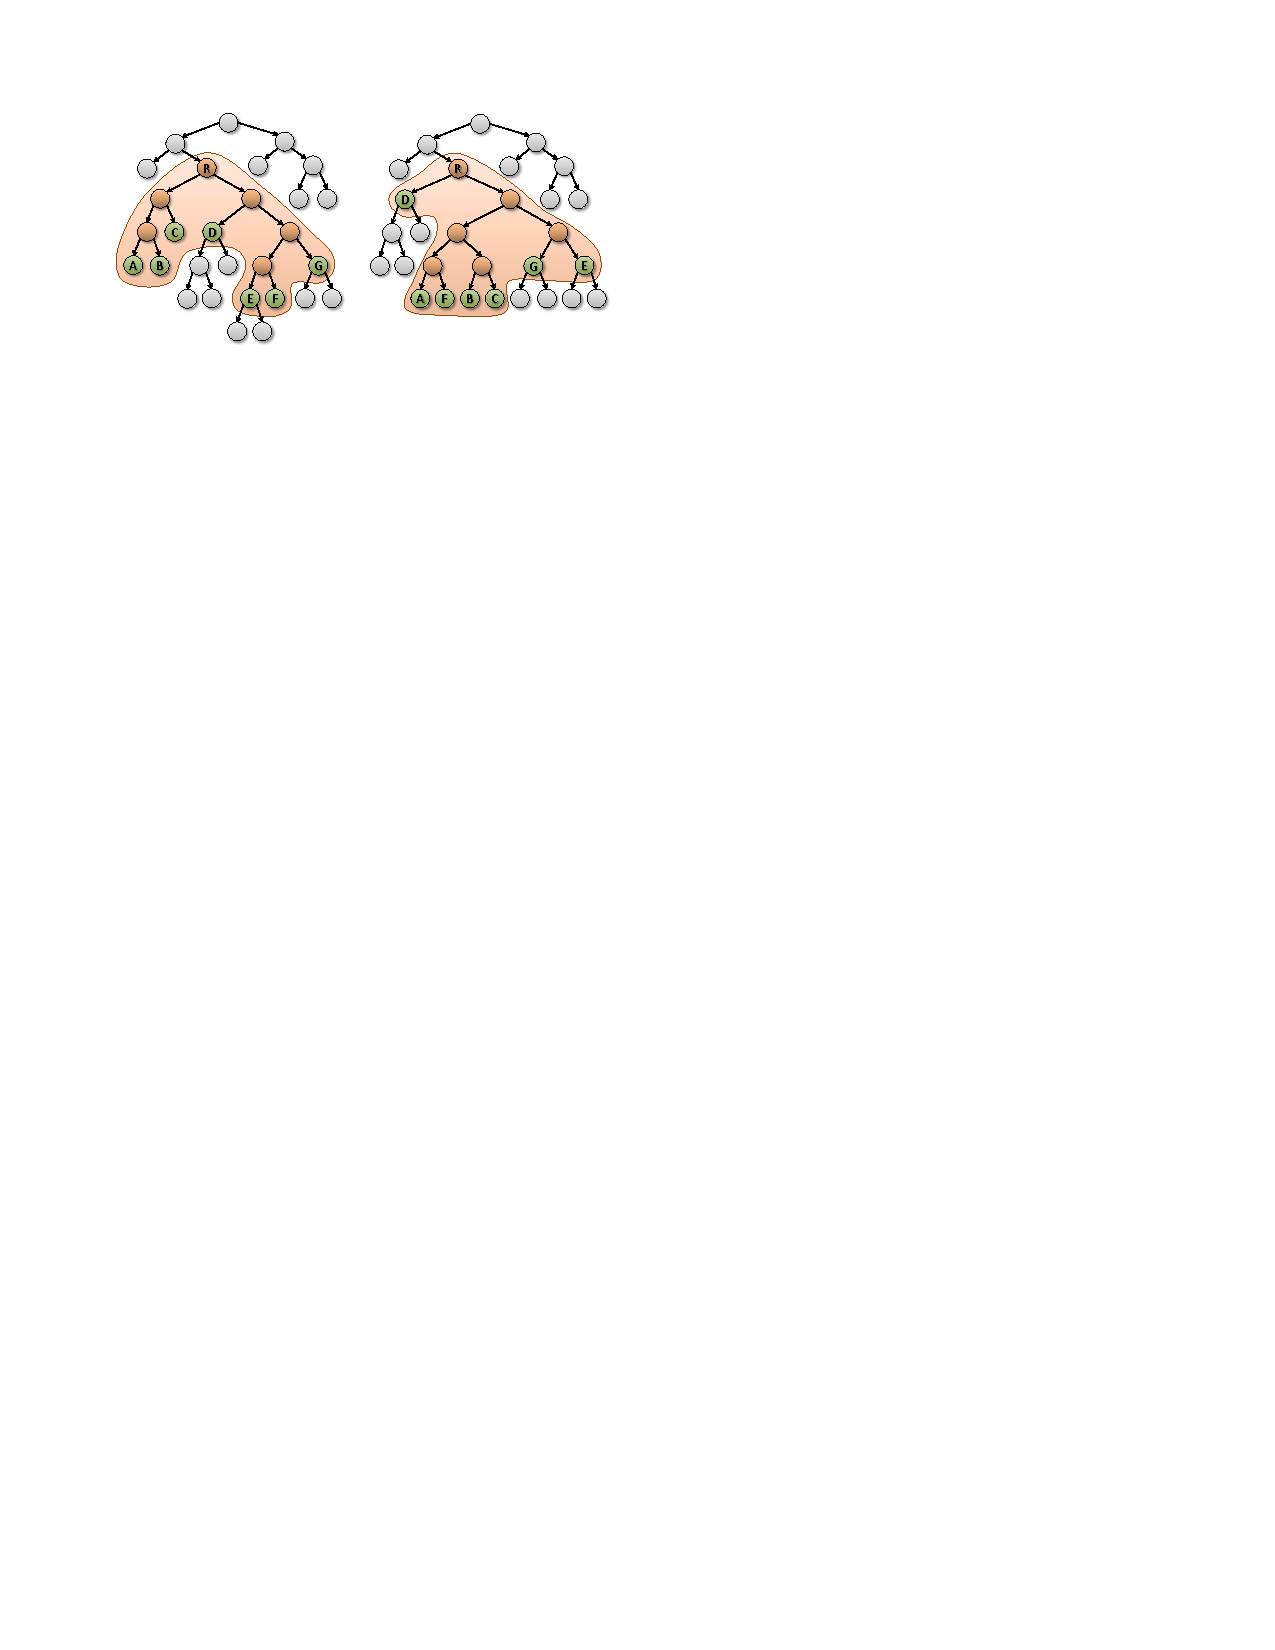
\psfig{file=tree.pdf,width =6in}
%\caption{A treelet rotation that decreases the ray tracing cost of the BVH~\cite{Karras:2013}.}
%\label{fig:treelet}
%\end{figure*}

%\begin{figure*}
%\centering
%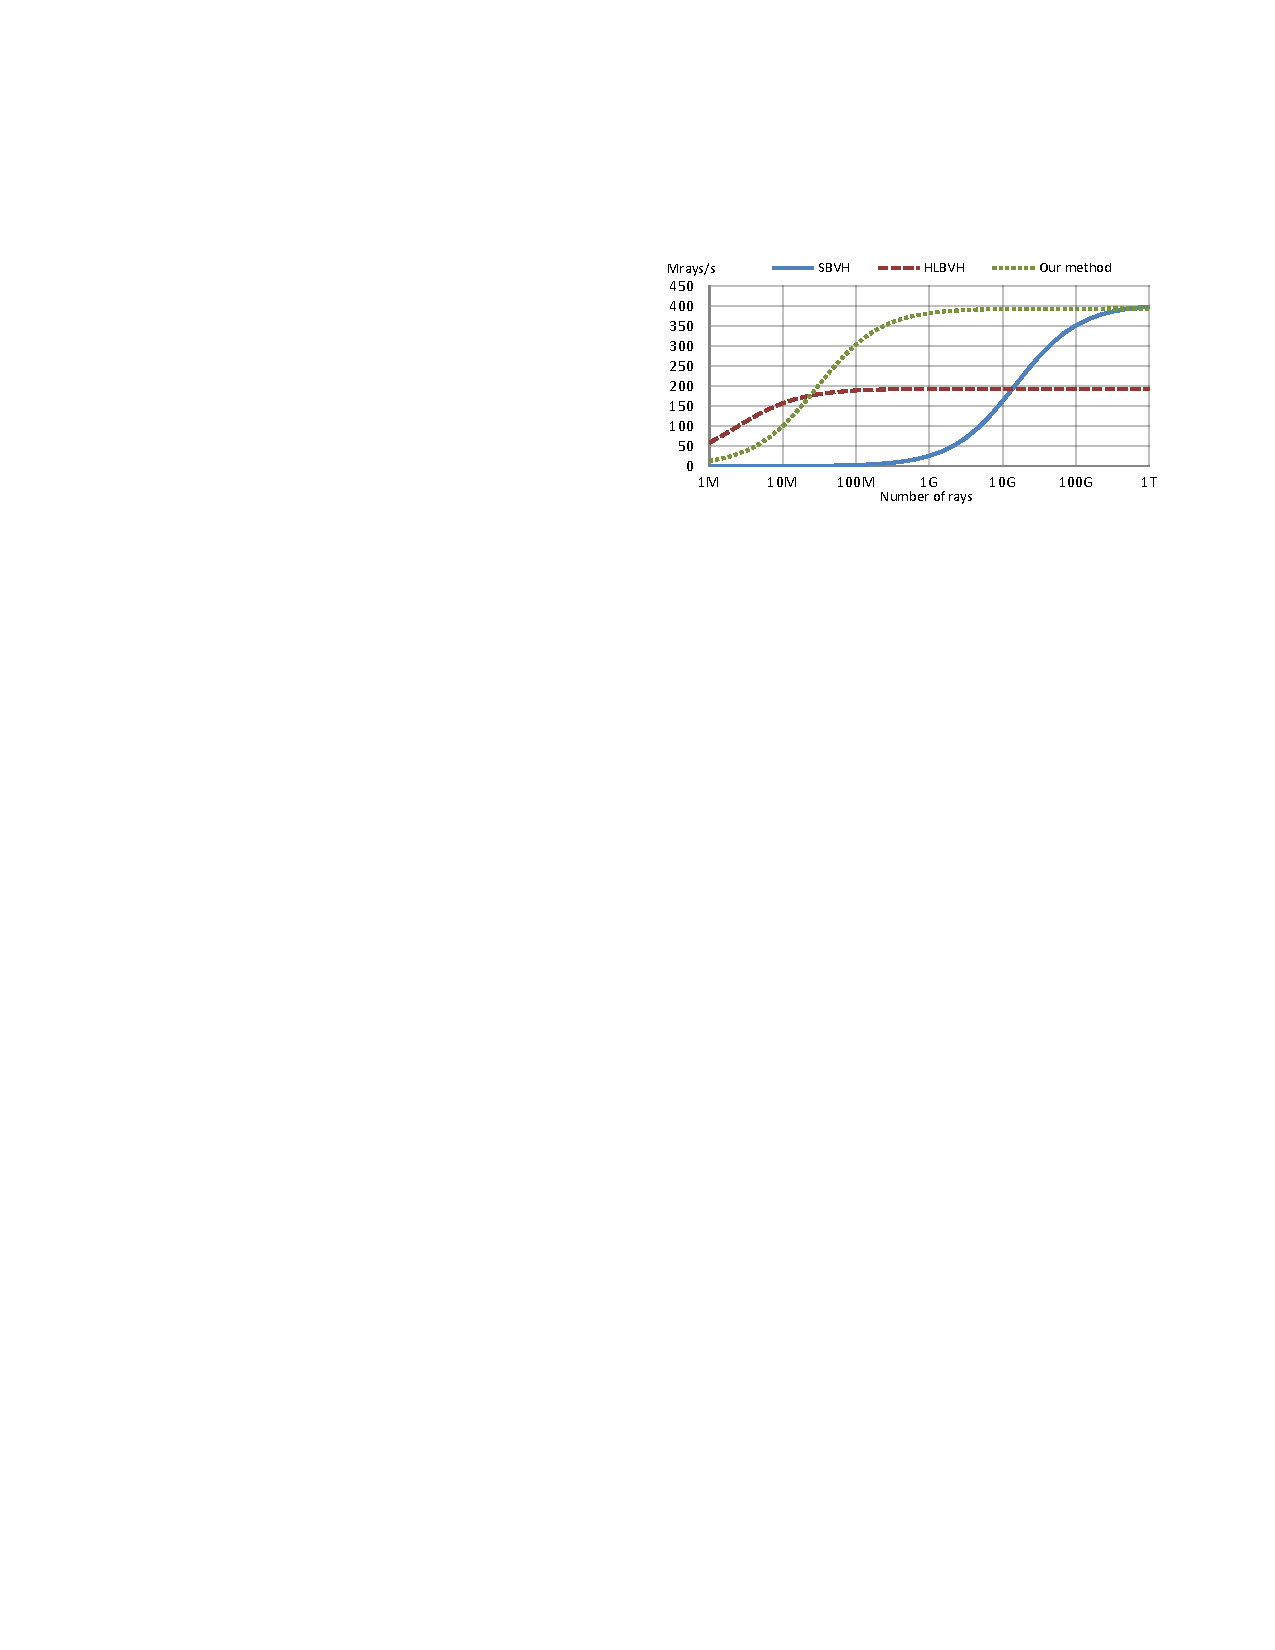
\psfig{file=graph.pdf,width =6in}
%\caption{Performance comparison from primary source~\cite{Karras:2013}.}
%\label{fig:treeletPerformance}
%\end{figure*}

%\todo[inline]{Needs more work}

\subsection{Results}
\label{sec:results}

As shown in Figure~\ref{fig:RadixCores}, the performance of the algorithm scales incredibly well as the number of cores increases. The execution time is inversely proportional to the number of cores. This is an excellent quality because the performance can be roughly doubled by doubling the number of cores assigned to the task~\cite{Karras:2012}. Figure~\ref{fig:RadixCores} also shows a comparison between this algorithm and the best previously known algorithm by Garanzha et al. As the number of cores increases, the new algorithm greatly surpasses the performance of the comparison method, even though the comparison method has elements of parallelism~\cite{Garanzha:2011}.

%Figure~\ref{fig:RadixPerformance} shows a comparison between this algorithm and the best previously known algorithm by Garanzha et al. It is apparent that the algorithm presented runs nearly twice as fast as the previous best. Additionally, the construction time is dominated by the sorting of primitives (shown as light green) rather than the hierarchy generation or AABB calculation. Conversely, the other algorithm appears to spend most of its time performing hierarchy generation.

\begin{figure}
\centering
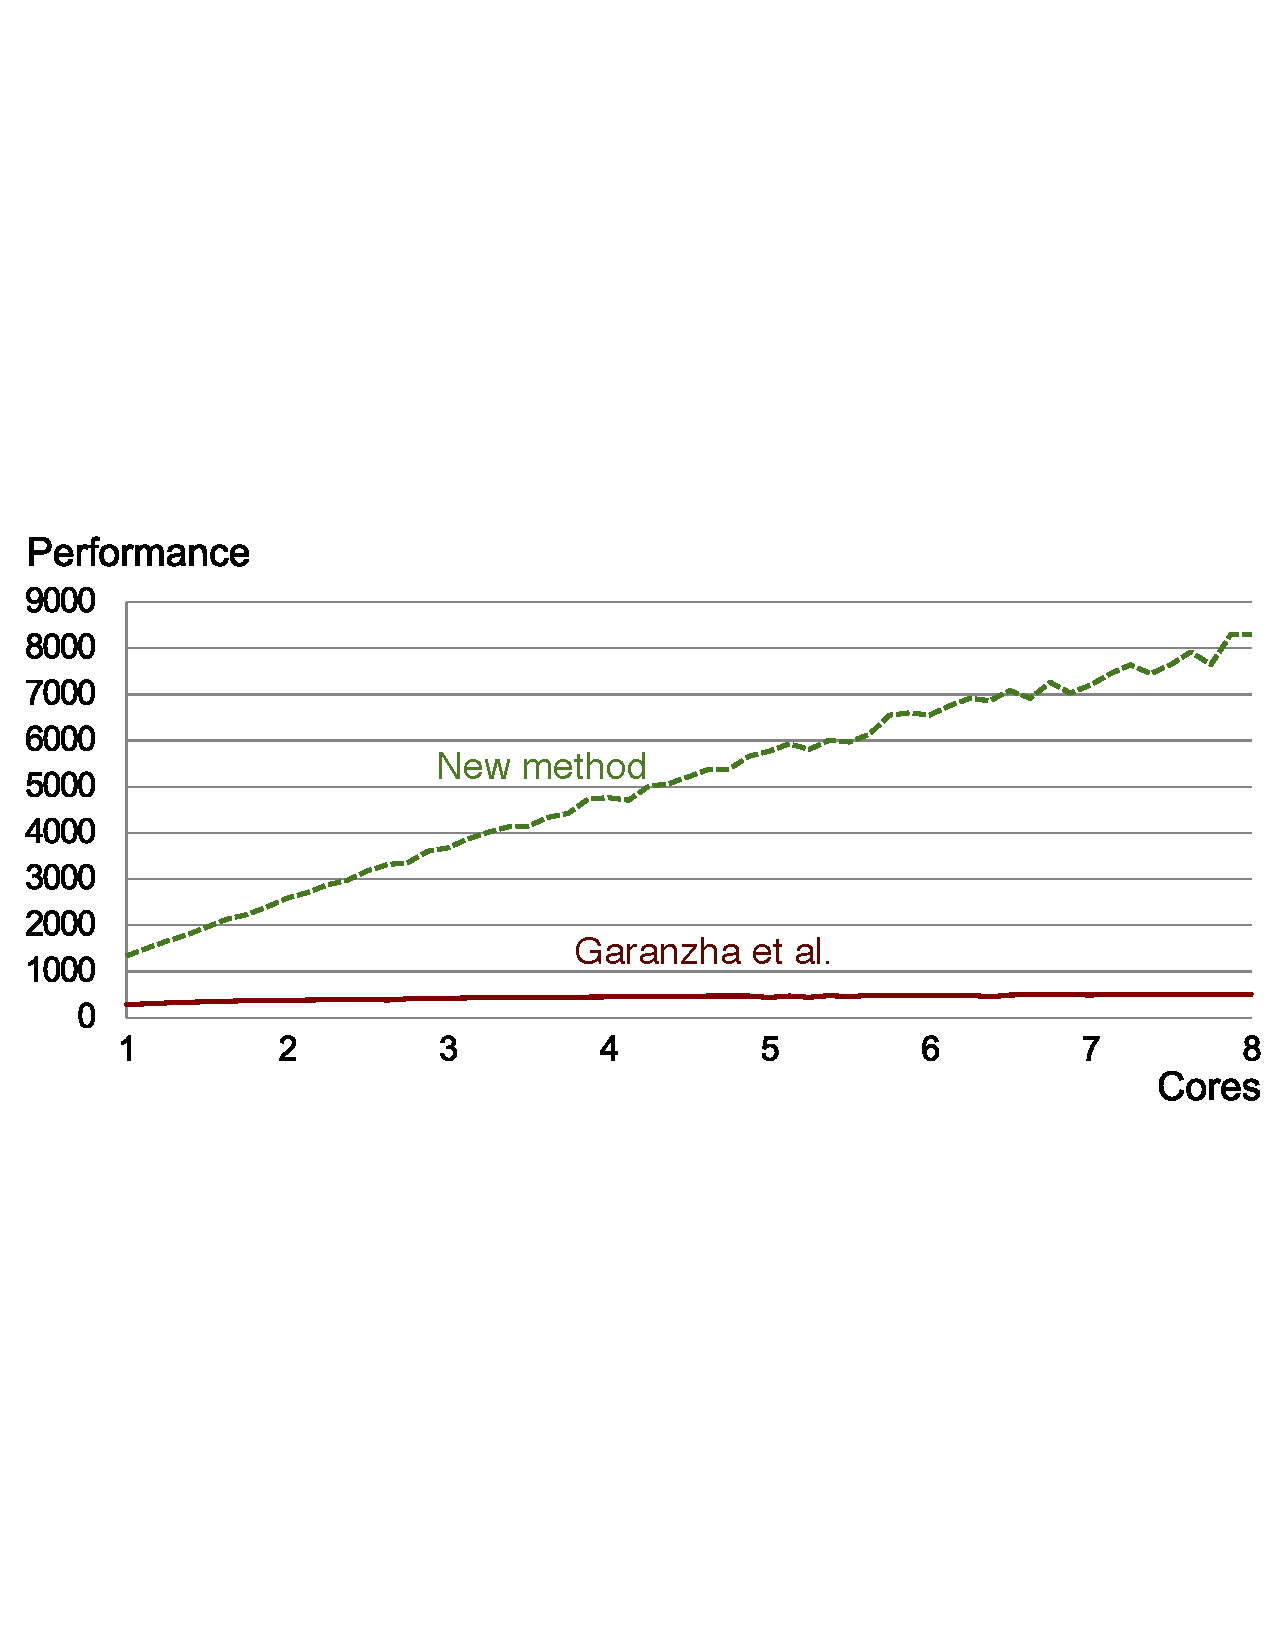
\psfig{file=cores.pdf,width =3in}
\caption{A comparison of two algorithms. The y axis represents millions of primitives per second and the x axis is the number of parallel cores.~\cite{Karras:2012}.}
\label{fig:RadixCores}
\end{figure}

\section{Conclusion}
\label{sec:conclusion}

The ray tracing technique is exceptional at producing high quality images of 3D scenes. The simulation of actual light propagation results in the shadows, reflections, and refractions which make images appear photorealistic. By using both the parallel BVH construction algorithm presented in this paper and hardware with multiple cores, real-time ray tracing becomes significantly faster. As the number of cores on modern hardware continues to increase, this algorithm will become even more impactful.

While this algorithm is a significant improvement over previous work, it is not without flaws. Scenes with poorly distributed primitives will generate BVHs that are not well-balanced. This is because the algorithm uses absolute locations of the primitives in the scene, rather than their positions relative to each other. An additional drawback to this algorithm is that it creates a new BVH for each frame without using any information from the previous frame. In sequences of frames where primitives move very little, it would be beneficial to simply adjust the previous frame's BVH, rather than constructing an entirely new one. Further research is needed to overcome these drawbacks. Overall, this research presents remarkable progress in the field of ray tracing.

%\begin{figure}
%\centering
%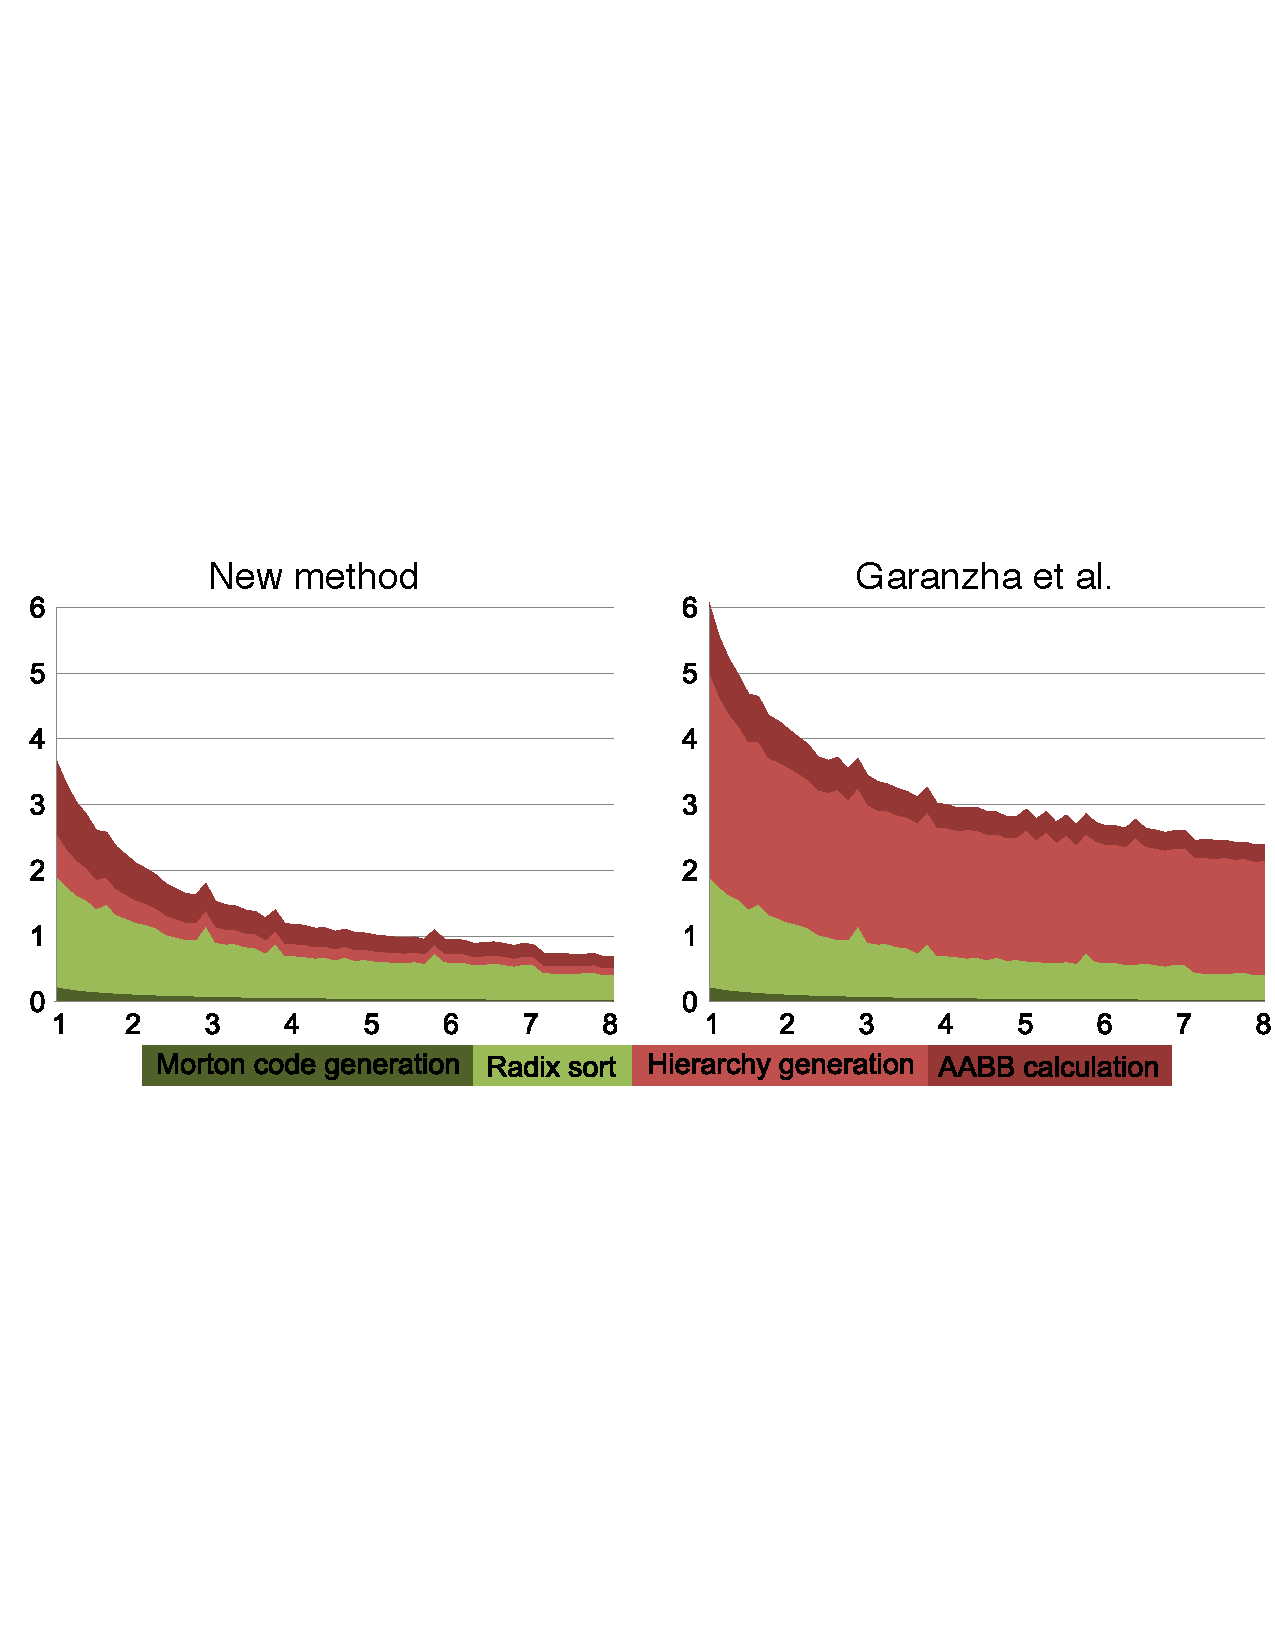
\psfig{file=performance.pdf,width =3in}
%\caption{A comparison of two algorithms for constructing a BVH for a sample scene.~\cite{Karras:2012}.}
%\label{fig:RadixPerformance}
%\end{figure}

\section*{Acknowledgments}
\label{sec:acknowledgments}

Thanks to Nic McPhee, Elena Machkasova, K.K. Lamberty, Max Magnuson, and Emma Sax for their time, feedback, and constructive comments.

% The following two commands are all you need in the
% initial runs of your .tex file to
% produce the bibliography for the citations in your paper.
\bibliographystyle{abbrv}
% sample_paper.bib is the name of the BibTex file containing the
% bibliography entries. Note that you *don't* include the .bib ending here.
\bibliography{ray_tracing}
% You must have a proper ".bib" file
%  and remember to run:
% latex bibtex latex latex
% to resolve all references

\end{document}
